\documentclass[12pt]{article}
\usepackage{amsmath}
\usepackage[top=0.5in, bottom=0.5in, left=0.5in, right=0.5in]{geometry}
\usepackage{multicol}
\usepackage{wrapfig}
\usepackage{listings}
\usepackage{enumerate}
\usepackage{graphicx}
\usepackage{parskip}
\usepackage{natbib}

\title{COMSM2127 -- Coursework 1}
\author{Chen Haoyan -- \texttt{candidate number:31288}}

\begin{document}

  \maketitle

  \vspace{-0.3in}
  \noindent
  \rule{\linewidth}{0.4pt}

  \noindent
%   \textbf{For each problem, briefly explain/justify how you
%   obtained your answer.} This will help us determine your understanding of
%   the problem whether or not you got the correct answer. Moreover, in the
%   event of an incorrect answer, we can still try to give you partial credit
%   based on the explanation you provide. It is fine for your answers to include
%   factorials, exponentials, or combinations; you don't need to calculate those
%   all out to get a single numeric answer.


%%%%%%%%%%%%%%%%%%%%%%%%%%%%%%%%%%%%%%%%%%%%%%%%%%%%%%%%%%%%%%%%%%%%%%%%%%%%%%%%
% Problems:

  \begin{enumerate}

    % Problem 1
    \item \textit{Simulate an integrate and fire model}
    
    The purpose in this question is to simulate and implement the \textbf{leaky integrate and fire model}. This model's formula is below:
    
    \begin{equation}
	  \tau_m\frac{dV}{dt}=E_L-V+R_mI_e
  	\end{equation}
    

    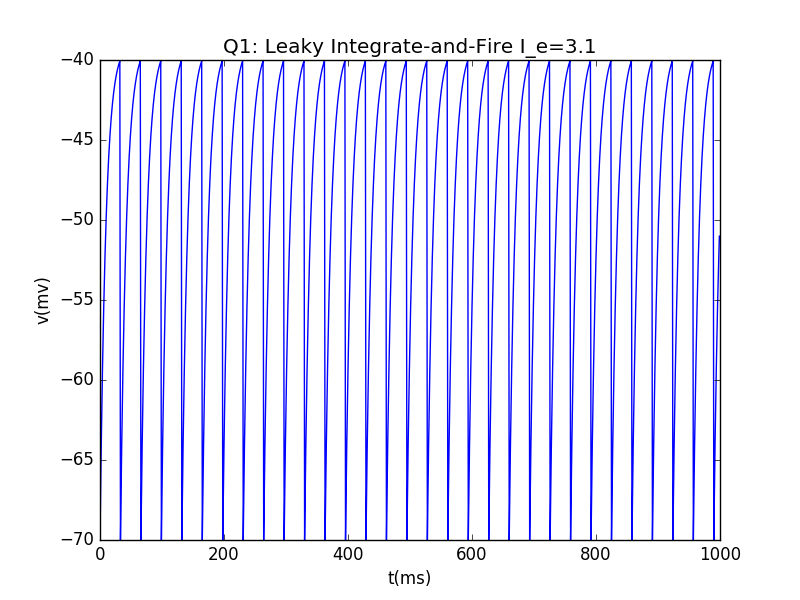
\includegraphics[width=0.5\linewidth]{figure_q1.png}
    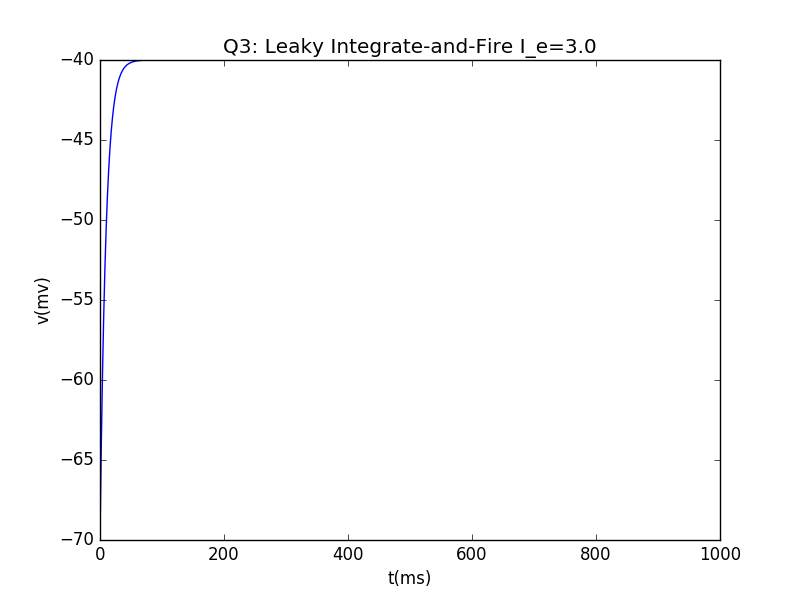
\includegraphics[width=0.5\linewidth]{figure_q3.png}

    We simulate this model for 1s, and as you can see in the left figure, the simulated neuron produces spikes or action potentials repeatedly when $I_e=3.1$.
          
    % Problem 2
    \item \textit{Compute analytically the minimum current $I_e$}
    
    From the equation (1) we can see that the value where $V$ stops changing, is
    \begin{equation}
    	\bar{V}=E_L+R_mI_e
    \end{equation}
    Hence, if $\bar{V}>V_{threshold}$ the neuron will generate spikes. Therefore, the $I_{threshold}$ should be
    \begin{equation}
        I_{threshold}=\frac{V_{threshold}-E_L}{R_m}
    \end{equation}
    Substituting the parameters in Question 1 to the equation (3), and then the result is $I_{threshold}=3.0$. So if $I_e>I_{threshold}$ (the minimum current $I_{minimum}=3.1$), the neuron will produce spikes.
    
    % Problem 3
    \item \textit{Simulate the neuron when $I_e=3.0$}
    
	The figure on the previous page shows the changing voltage of the neuron when $I_e$ equals 3.0. Other parameters are as same as those in question 1. As shown in the figure above, there is no spikes when $I_e=3.0$. In other words, the voltage have never reached $V_T$.
    
    % Problem 4
    \item \textit{F-I curve}
    
    Obviously we just try to change the value of $I_e$ from 2 [nA] to 5 [nA] in steps of 0.1 [nA], and count the number of spikes. As shown in the following figure, there is no firing until the input current is larger than 3.0.
    \begin{center}
    	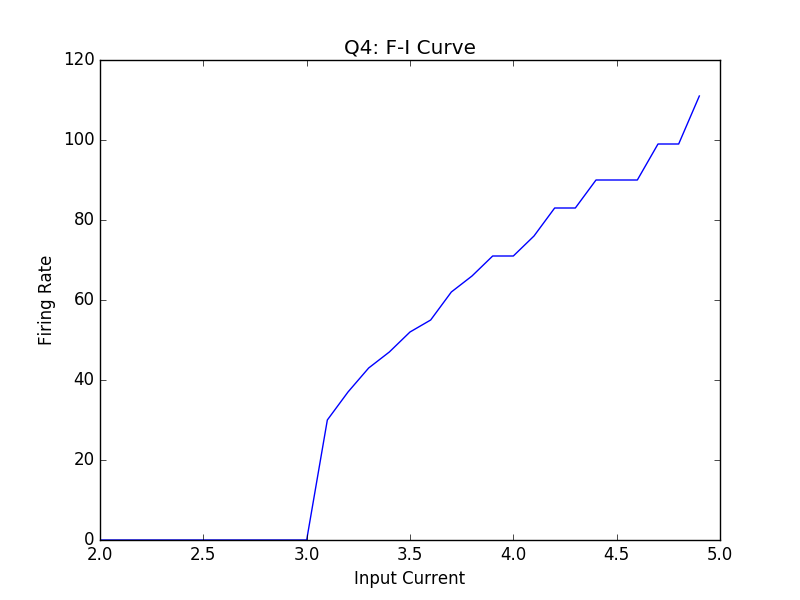
\includegraphics[width=0.5\linewidth]{figure_q4.png}
	\end{center}
    
    % Problem 5
    \item \textit{Simulate synaptic connections (simple synapse model) }
    
    The neurons are coupled through synaptic currents, so these two neurons should satisfy the following equations
    \begin{equation}
    	\tau_m\frac{dV_1}{dt}=E_L-V_1+R_mI_e+R_m\bar{g_s}S_2(E_s-V_1)
    \end{equation}
    \begin{equation}
    	\tau_s\frac{dS_2}{dt}=-S_2
    \end{equation}
    with other two equations with 1 and 2 swapped. 
    
    $$
    \begin{cases}
    V_1=V_r, S_1->S_1+P & V_1>V_t\\
    V_2=V_r, S_2->S_2+P & V_2>V_t
    \end{cases}
    $$
    
    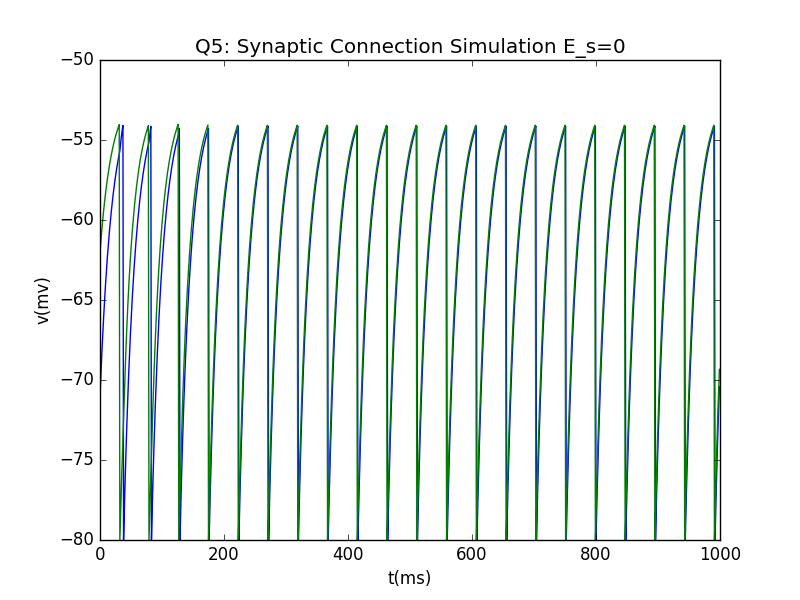
\includegraphics[width=0.5\linewidth]{figure_q5_1.png}
    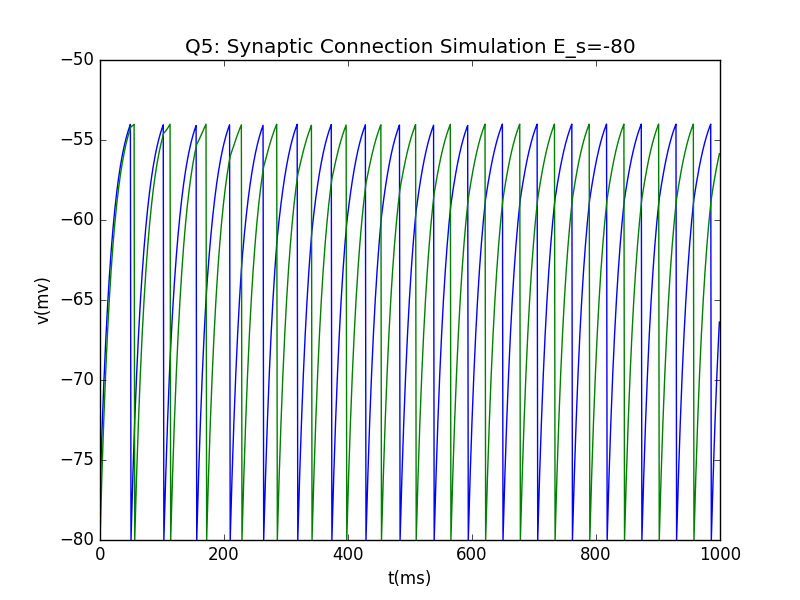
\includegraphics[width=0.5\linewidth]{figure_q5_2.png}
    
    The excitatory synaptic connections are simulated in the left figure. As we can see from this graph, the changing voltage of those two neurons are similar through excitatory synaptic connections. However, in the right figure, the variation of the neurons' voltage are inhibitory to each other. In other words, the inhibitory synapse makes a postsynaptic neuron less likely to generate an action potential.

	% Problem 6
    \item \textit{Simulate potassium current  }
    
    In this question, we only simulate one neuron whose firing rate falls off after the first spike. In the following equations, $R_mg_k(E_k-V)$ simulates a slow potassium current. If the neuron produces a spike, $g_k$ should increase by 0.005  $(M\Omega)^{-1}$ ($g_k->g_k+dg_k$, $dg_k=0.005$). Otherwise, it should decay by equation (7). 
    
    \begin{equation}
    \tau_m\frac{dV}{dt}=E_L-V+R_mI_e+R_mg_k(E_k-V)
    \end{equation}
    \begin{equation}
    \tau_k\frac{dg_k}{dt}=-g_k
    \end{equation}
    
    
    \begin{center}
    	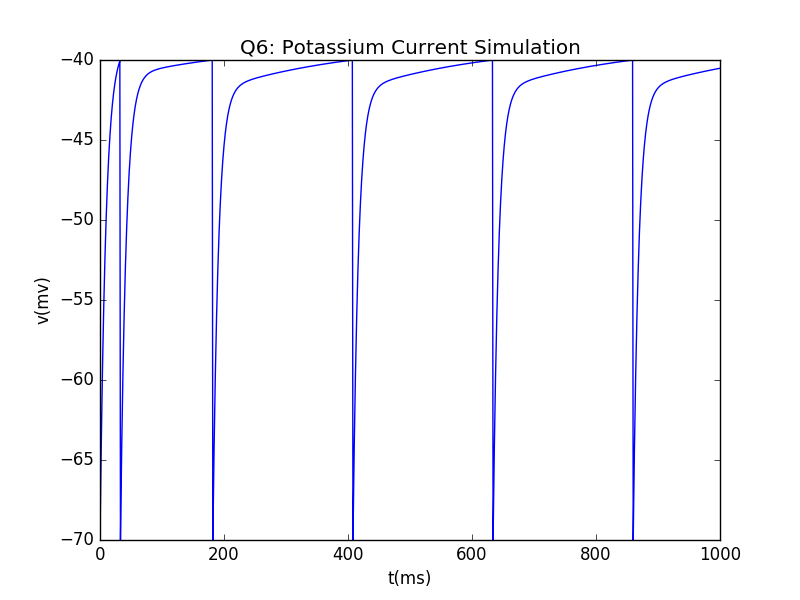
\includegraphics[width=0.5\linewidth]{figure_q6.png}
    \end{center}
    
    
    % Problem 7
    \item \textit{Synaptic connections (Alpha function)  }
    
    From the following equation, we can see that the alpha function describes a conductance that has a rising phase that is not infinitely fast, but has a certain rise time\citep{roth2009modeling}. 
    \begin{equation}
    	g_{syn}(t)=\bar{g}_{syn}\frac{t-t_0}{\tau}e^{1-(t-t_0)/\tau}
    \end{equation}
    
    Hence, in my opinion, if we apply the alpha function model to the synaptic connections, the rising phases of voltage curves will be smoother than those in the figures of question 5.

  \end{enumerate}
  
\bibliographystyle{plain} % or try abbrvnat or unsrtnat
\bibliography{export} % refers to example.bib
\end{document}